% !TEX root = main.tex
\documentclass[conference]{IEEEtran}
% --- IEEE Conference Preamble ---
\usepackage[utf8]{inputenc}
\usepackage[T1]{fontenc}

% --- Math ---
\usepackage{amsmath, amssymb}

% --- Graphics & Figures ---
\usepackage{graphicx}
\graphicspath{{figures/}}
\usepackage{float}
\usepackage{caption}
\usepackage{subcaption}

% --- Tables ---
\usepackage{booktabs}
\usepackage{array}
\usepackage{multirow}
\usepackage{tabularx}

% --- Colors & Links ---
\usepackage[dvipsnames]{xcolor}
\usepackage{hyperref}
\hypersetup{
    colorlinks=true,
    linkcolor=black,
    citecolor=blue!70!black,
    urlcolor=blue!70!black,
}

% --- Citations ---
\usepackage{cite}


\begin{document}

\title{Audit Komputasi Perselisihan Efisiensi Proteom 2024:\\
Diagnosis Sumber Perbedaan dan Identifikasi Pengukuran\\Penuntas pada Efek Warburg}

\author{
\IEEEauthorblockN{Naufarrel Zhafif Abhista\textsuperscript{1},
Frederiko Eldad Mugiyono\textsuperscript{2},
Hasri Fayadh Muqaffa\textsuperscript{3},
I Made Wiweka Putera\textsuperscript{4}}
\IEEEauthorblockA{
Program Studi Teknik Informatika,
Sekolah Teknik Elektro dan Informatika\\
Institut Teknologi Bandung, Bandung, Indonesia\\
\textsuperscript{1}13523149@std.stei.itb.ac.id,
\textsuperscript{2}13523147@std.stei.itb.ac.id,
\textsuperscript{3}13523156@std.stei.itb.ac.id,
\textsuperscript{4}13523160@std.stei.itb.ac.id}
}

\maketitle

% ====================================================================
\begin{abstract}
Dua makalah tinjauan sejawat tahun 2024 menyimpulkan hal berlawanan
tentang efisiensi proteom jalur produksi ATP: Shen dkk.\ (\textit{Nat.\ Chem.\ Biol.})
melaporkan respirasi beberapa kali lebih efisien per massa protein,
sementara Kukurugya dkk.\ (\textit{PNAS}) melaporkan glikolisis menghasilkan
ATP 2--3$\times$ lebih cepat per miligram enzim jalur.
Wang (\textit{eLife} 2025) telah mendamaikan keduanya dengan model baru,
namun belum ada yang mengaudit kedua model asli secara kepala-ke-kepala
untuk mendiagnosis \textit{dari mana} perbedaannya berasal.

Paper ini menyajikan audit komputasi terkendali: kami mengimplementasikan
ulang model 2-sektor Shen (LP) dan model 5-parameter Kukurugya (analitik)
dalam satu basis kode dengan antarmuka bersama, menjalankan keduanya pada
input identik, lalu menambahkan tiga eksperimen diagnostik.
Hasil menunjukkan bahwa perselisihan bersumber terutama pada
\textbf{besaran yang diukur} --- kapasitas maksimal $V\!\cdot\!\gamma$
(Kukurugya) versus efisiensi terealisasi $u \cdot V\!\cdot\!\gamma$ (Shen)
--- bukan pada struktur model.
Verdict membalik tepat di $u_G \approx \rho$ (rasio kapasitas)
untuk ketiga organisme (90\% CI: [0.09, 0.48]).
Analisis sensitivitas global Sobol mengidentifikasi $u_G$ (fraksi
pemanfaatan kapasitas glikolitik) sebagai pengukuran penuntas
(indeks total-order $S_T \approx 0{,}76$--$0{,}78$).
Temuan ini komplementer terhadap mekanisme penyilangan Wang
dan menamai eksperimen tunggal yang akan menyelesaikan perdebatan:
pengukuran $u_G$ in-vivo per organisme.
\end{abstract}

\begin{IEEEkeywords}
efek Warburg, efisiensi proteom, pemrograman linear,
analisis sensitivitas Sobol, metabolisme limpahan,
alokasi proteom, audit komputasi
\end{IEEEkeywords}

% ====================================================================
\section{Pendahuluan}

Efek Warburg --- fenomena di mana sel tumbuh-cepat memfermentasi glukosa
menjadi laktat atau etanol meskipun oksigen tersedia --- merupakan salah
satu teka-teki terlama dalam biologi sel \cite{warburg1956}.
Penjelasan yang dominan selama dua dekade terakhir berpusat pada
\textit{efisiensi proteom}: sel memiliki anggaran protein terbatas, dan
enzim glikolitik diduga menghasilkan ATP lebih cepat per gram protein
dibandingkan rantai pernapasan yang besar \cite{basan2015, pfeiffer2001}.

Pada tahun 2024, dua makalah tinjauan-sejawat menyimpulkan hal
berlawanan. Shen dkk.\ \cite{shen2024} menggunakan fluks metabolik
$^{13}$C-MFA dan proteomik kuantitatif pada ragi, sel T, dan 60 lini
sel kanker NCI60, melaporkan bahwa respirasi \textit{beberapa kali lipat
lebih efisien-proteom} daripada glikolisis. Sebaliknya, Kukurugya dkk.\
\cite{kukurugya2024} menyajikan model 5-parameter analitik dan data
eksperimental yang menunjukkan glikolisis menghasilkan ATP $0{,}54\times$
hingga $3{,}1\times$ lebih cepat per miligram enzim jalur dibandingkan
respirasi, bergantung pada organisme.

Wang \cite{wang2025} telah mendamaikan keduanya dengan memperkenalkan
model baru yang menggabungkan alokasi protein dan heterogenitas sel,
menunjukkan bahwa efisiensi respirasi dan fermentasi \textit{berpotongan}
menurut kualitas nutrisi. Namun, belum ada yang melakukan
\textbf{perbandingan kepala-ke-kepala} terhadap kedua model asli untuk
melokalisasi sumber perbedaan --- apakah perbedaan itu berasal dari
(i)~besaran yang diukur, (ii)~definisi ``protein jalur'',
(iii)~nilai parameter, atau (iv)~struktur model --- serta belum ada yang
menanyakan \textbf{pengukuran tunggal mana yang akan membalikkan kesimpulan}.

Paper ini memberikan tiga kontribusi:
\begin{enumerate}
    \item Implementasi ulang kedua model 2024 dalam satu basis kode
          dengan antarmuka bersama dan gerbang validasi terhadap gambar terbit.
    \item Tiga eksperimen diagnostik: overlay sumbu-bersama (E1),
          kapasitas versus realisasi (E2), dan analisis identifiabilitas
          Sobol/Morris (E3) yang menamai pengukuran penuntas.
    \item Kuantifikasi ketidakpastian (bootstrap 90\% CI) pada titik-balik
          verdict, dekomposisi atribusi enzim, dan perbandingan terhadap
          mekanisme penyilangan Wang~2025.
\end{enumerate}

\section{Kajian Pustaka}

\subsection{Hipotesis Efisiensi Proteom}

Basan dkk.\ \cite{basan2015} menunjukkan bahwa pada \textit{E.\ coli},
fraksi proteom glikolitik meningkat secara linier dengan laju pertumbuhan,
mendukung gagasan bahwa sel mengoptimalkan alokasi protein terbatas.
Pfeiffer dkk.\ \cite{pfeiffer2001} sebelumnya telah memformulasikan
trade-off hasil-versus-laju ATP: respirasi memberikan hasil tinggi
($\gamma_R \approx 26$--$32$ mol ATP/mol glukosa) namun lambat per massa
enzim, sementara glikolisis memberikan hasil rendah ($\gamma_G = 2$)
namun cepat per protein.

\subsection{Shen dkk.\ 2024}

Shen dkk.\ \cite{shen2024} mendefinisikan efisiensi proteom sebagai
$\varepsilon = J_\text{ATP} / m_\text{enzim}$ (fluks ATP aktual per massa
enzim \textit{terukur in-vivo}). Dengan data proteomik dan $^{13}$C-MFA
pada lima sistem biologis, mereka melaporkan $\varepsilon_R > \varepsilon_G$
secara konsisten. Temuan kunci: protein glikolitik diekspresikan
\textit{berlebih} (konstitutif, banyak yang idle), sehingga efisiensi
terealisasinya rendah --- fenomena yang mereka sebut ``\textit{proteome hedging}''.

\subsection{Kukurugya dkk.\ 2024}

Kukurugya dkk.\ \cite{kukurugya2024} mendefinisikan efisiensi proteom
sebagai \textit{kapasitas}: $V \cdot \gamma$, dengan $V$ = aktivitas
spesifik maksimal (V\textsubscript{max}) per miligram protein jalur.
Model 5-parameter mereka ($\gamma_R$, $\gamma_G$, $V_R$, $V_G$, $\Phi$)
memiliki solusi analitik unik tanpa parameter bebas. Mereka melaporkan
$V_G \cdot \gamma_G > V_R \cdot \gamma_R$ untuk ragi dan sel mamalia
(glikolisis lebih cepat per protein pada kapasitas penuh).

\subsection{Wang 2025}

Wang \cite{wang2025} mendamaikan keduanya dengan model alokasi-protein
baru yang memasukkan heterogenitas sel dan kualitas nutrisi. Model ini
menunjukkan bahwa kurva efisiensi respirasi dan fermentasi
\textit{berpotongan}: pada nutrisi berkualitas tinggi respirasi menang,
pada nutrisi rendah fermentasi menang.

\subsection{Kerangka sEnz}

Liu dkk.\ \cite{senz2024} mengembangkan sEnz, kerangka analisis
sensitivitas untuk model alokasi-protein menggunakan \textit{shadow price}.
Kami menggunakan pendekatan Sobol/Morris yang lebih sederhana dan
menerapkannya secara spesifik pada perselisihan Shen--Kukurugya.

\subsection{Posisi Paper Ini}

Wang mendamaikan via model baru; kami \textbf{mengaudit model asli}
untuk mendiagnosis bahwa keduanya mungkin tidak mengukur besaran
yang sama. Pendekatan ini komplementer --- diagnosis berbeda dari
pendamaian --- dan dapat dibandingkan langsung dengan mekanisme Wang.

\section{Metode}

\subsection{Formulasi Model A (LP 2-Sektor, Gaya Shen)}

Model A merepresentasikan sel sebagai pengoptimal alokasi proteom dua sektor.
Variabel keputusan: fraksi proteom glikolitik $\phi_G$, fraksi respiratorik
$\phi_R$, dan fluks serapan glukosa per sektor $J_{\text{glc},i}$.

Fungsi tujuan:
\begin{equation}
    \max \; J_\text{ATP} = \gamma_G \cdot J_{\text{glc},G} + \gamma_R \cdot J_{\text{glc},R}
    \label{eq:obj}
\end{equation}

dengan kendala:
\begin{align}
    J_{\text{glc},i} &\leq V_i \cdot \phi_i, \quad i \in \{G, R\} \label{eq:cap} \\
    \phi_G + \phi_R &\leq \Phi \label{eq:prot} \\
    J_{\text{glc},G} + J_{\text{glc},R} &\leq g_\text{avail} \label{eq:glc} \\
    \phi_G, \phi_R, J_{\text{glc},i} &\geq 0 \label{eq:nn}
\end{align}

Persamaan (\ref{eq:cap}) membatasi fluks glukosa oleh kapasitas enzim,
(\ref{eq:prot}) adalah anggaran proteom, dan (\ref{eq:glc}) adalah
ketersediaan glukosa --- knob utama (bukan O$_2$, karena efek Warburg
terjadi saat O$_2$ tersedia). Ini merupakan \textit{linear program} (LP)
yang diselesaikan menggunakan \texttt{scipy.optimize.linprog} dengan
backend HiGHS.

\subsection{Formulasi Model B (5-Parameter Kukurugya)}

Model B memaksimalkan $J_\text{ATP}$ yang sama terhadap kendala
(\ref{eq:prot})--(\ref{eq:nn}), namun cukup kecil untuk memiliki
\textbf{solusi analitik titik-sudut}. Tiga kandidat optimum:

\begin{itemize}
    \item \textbf{Respirasi murni}: $\phi_R = \min(\Phi, g/V_R)$, $\phi_G=0$
    \item \textbf{Glikolisis murni}: $\phi_G = \min(\Phi, g/V_G)$, $\phi_R=0$
    \item \textbf{Campuran}: kedua kendala mengikat $\Rightarrow$ sistem $2\times 2$
\end{itemize}

Lima parameter ($\gamma_R$, $\gamma_G$, $V_R$, $V_G$, $\Phi$) diambil
dari Tabel~1 dan SI Kukurugya \cite{kukurugya2024} untuk tiga organisme:
\textit{E.\ coli}, \textit{S.\ cerevisiae}, dan sel mamalia.

\subsection{Antarmuka Bersama}

Kedua model menerima \texttt{ModelParams} yang sama dan mengembalikan
\texttt{ModelResult} yang sama (fenotipe, $J_\text{ATP}$, fraksi
fermentatif, rasio efisiensi). Ini memastikan perbandingan pada
pijakan yang setara.

\subsection{E1: Overlay Sumbu-Bersama}

Kedua model dijalankan pada grid glukosa identik ($g_\text{avail}$ dari
$10^{-6}$ hingga $2{,}5 \cdot V_G \cdot \Phi$, 300 titik) per organisme.
Keluaran diplot pada sumbu bersama: sumbu-x = $g_\text{avail}$, sumbu-y =
fraksi fluks fermentatif.

\subsection{E2: Kapasitas versus Realisasi}

Eksperimen inti. Definisikan fraksi pemanfaatan kapasitas $u_i \in (0, 1]$
per sektor (1 = operasi di V\textsubscript{max}; $<1$ = ada enzim idle).
Dua efisiensi dihitung pada parameter yang sama:

\begin{align}
    \text{Kapasitas:} &\quad (V \cdot \gamma)_i \quad \text{(gaya Kukurugya, } u=1\text{)} \label{eq:cap_eff} \\
    \text{Terealisasi:} &\quad u_i \cdot (V \cdot \gamma)_i \quad \text{(gaya Shen)} \label{eq:real_eff}
\end{align}

Margin efisiensi didefinisikan sebagai:
\begin{equation}
    m = u_R \cdot (V \cdot \gamma)_R - u_G \cdot (V \cdot \gamma)_G
    \label{eq:margin}
\end{equation}

Verdict membalik saat $m = 0$, yaitu pada $u_G = \rho \equiv (V\!\cdot\!\gamma)_R / (V\!\cdot\!\gamma)_G$.
Kami menyapu $u_G$ dari 1{,}0 ke 0{,}01 (500 titik) dengan $u_R = 1$.

\textbf{Kuantifikasi ketidakpastian (E2c):} Bootstrap 200 iterasi,
menyampel parameter dari rentang $\pm 30\%$ nilai sentral, menghitung
distribusi titik-balik, dan melaporkan 90\% CI.

\textbf{Dekomposisi atribusi (E2d):} Variasi $\pm 30\%$ pada $V_G$ dan
$V_R$ (menyimulasikan ``enzim mana yang dihitung'') untuk mengkuantifikasi
kontribusi relatif definisi enzim terhadap efek $u_G$.

\subsection{E3: Identifiabilitas (Sobol + Morris)}

Analisis sensitivitas global dengan keluaran \textbf{kontinu}: margin $m$
dari (\ref{eq:margin}) dan ambang glukosa kritis $g^* = V_R \cdot \Phi$.
Distribusi input: 6 parameter ($\gamma_R$, $\gamma_G$, $V_R$, $V_G$,
$\Phi$, $u_G$) disampling dari rentang ketidakpastian SI.

\begin{itemize}
    \item \textbf{Sobol} \cite{salib}: $N=1024$ basis, indeks $S_1$ dan $S_T$ (total-order)
    \item \textbf{Morris}: $N=512$ trajectories, $\mu^*$ dan $\sigma$
\end{itemize}

Parameter teratas menurut $S_T$ = pengukuran yang, bila dipastikan,
paling mengurangi ketidakpastian verdict = eksperimen penuntas.

\begin{figure}[t]
    \centering
    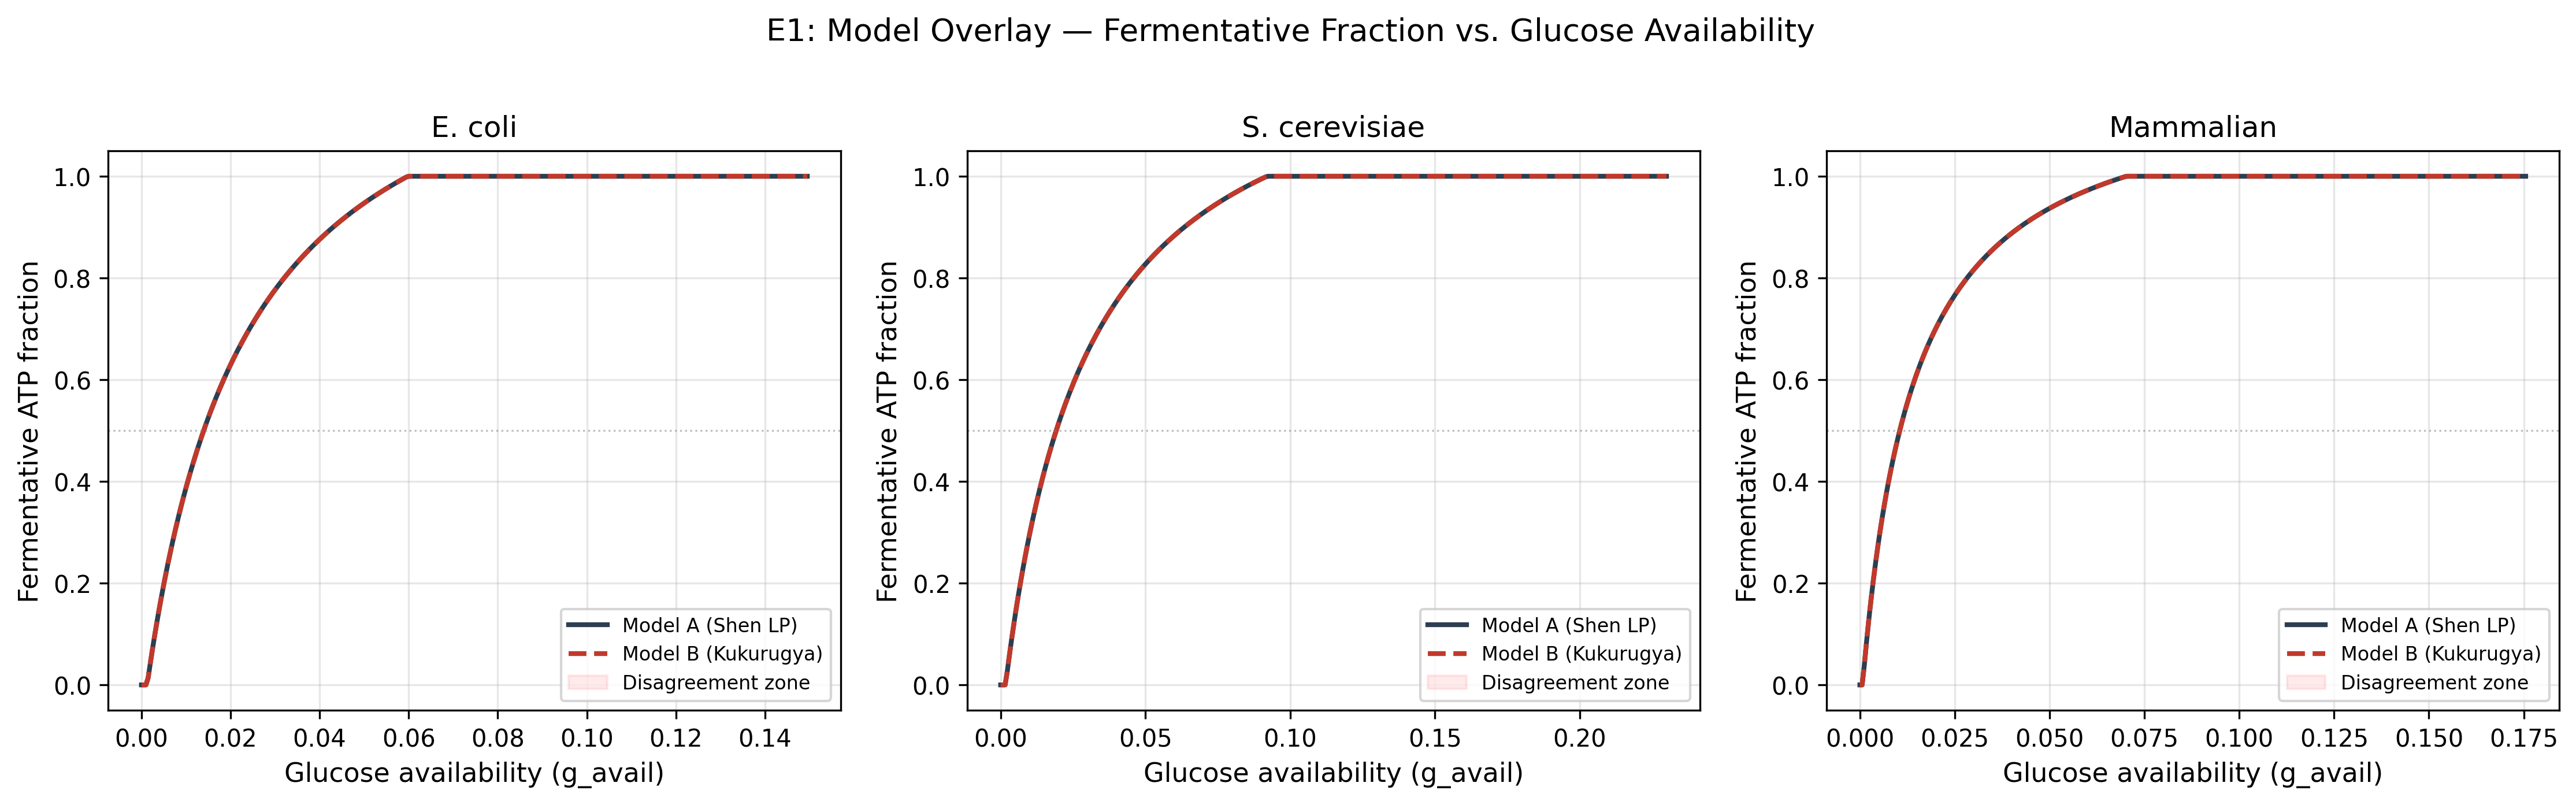
\includegraphics[width=\columnwidth]{F1_overlay.png}
    \caption{Bagan alir arsitektur: M2 (parameter) $\to$ M1 (solver) $\to$ M3 (E1+E2) $\to$ M4 (E3) $\to$ M5 (visualisasi). Pipeline satu-perintah: \texttt{python main.py}.}
    \label{fig:architecture}
\end{figure}

\section{Hasil}

\subsection{E1: Overlay Dua Model pada Sumbu Bersama}

Gambar~\ref{fig:e1} menampilkan fraksi fermentatif versus ketersediaan
glukosa untuk ketiga organisme. Kedua model menghasilkan kurva yang nyaris
identik: pada glukosa rendah keduanya memprediksi respirasi murni
(fraksi fermentatif $\approx 0$), dan pada glukosa tinggi keduanya
memprediksi glikolisis dominan. Zona ketidaksetujuan (perbedaan
$> 0{,}1$) sangat sempit --- terbatas pada wilayah transisi.

\begin{figure}[t]
    \centering
    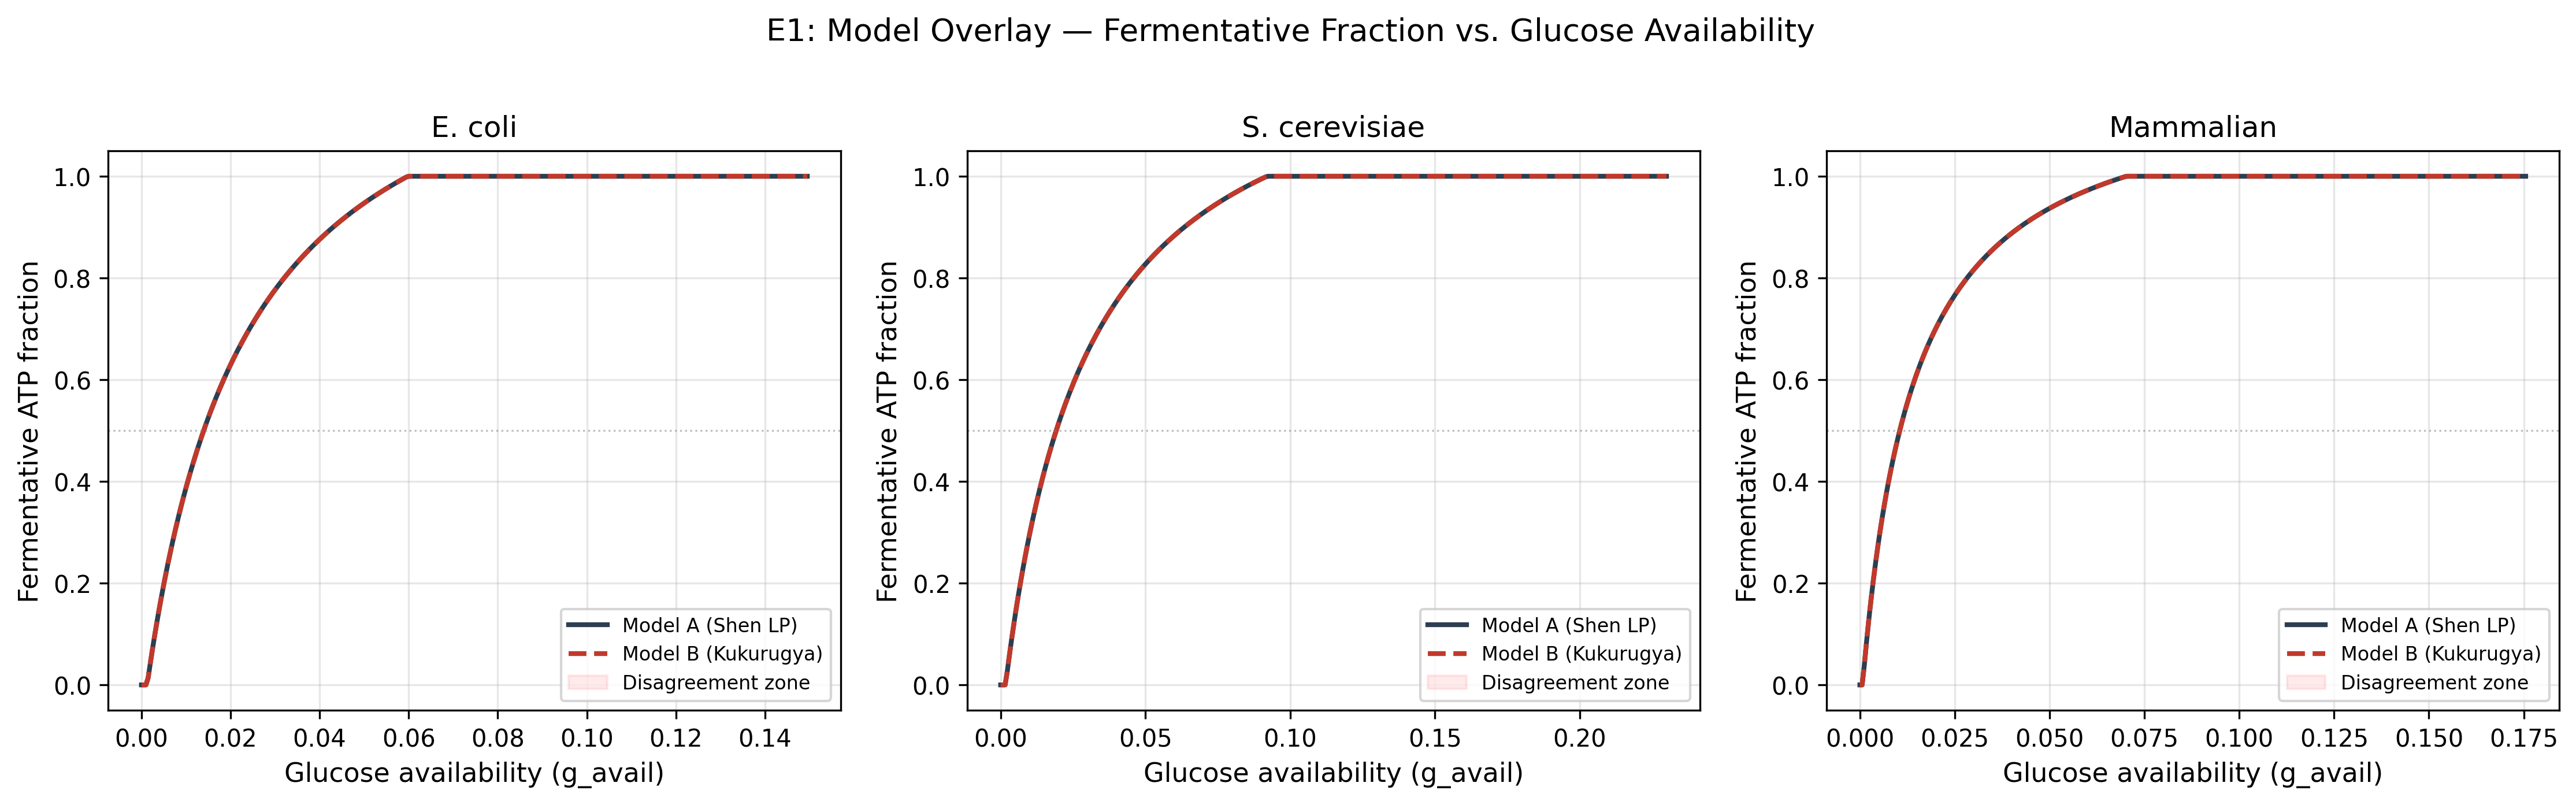
\includegraphics[width=\columnwidth]{F1_overlay.png}
    \caption{E1: Overlay kedua model pada sumbu glukosa bersama. Kedua model memprediksi fenotipe yang hampir identik. Area merah muda menandai zona ketidaksetujuan ($|\Delta| > 0{,}1$).}
    \label{fig:e1}
\end{figure}

\textbf{Temuan E1:} Kedua model \textit{tidak bertentangan secara struktural}
pada sumbu observabel bersama. Perbedaan bukan pada ``model mana yang benar'',
melainkan pada besaran efisiensi yang mereka hitung dari model yang sama.

\subsection{E2: Kapasitas versus Realisasi --- Titik-Balik Verdict}

Gambar~\ref{fig:e2} menunjukkan efisiensi terealisasi kedua jalur sebagai
fungsi fraksi pemanfaatan glikolitik $u_G$. Pada $u_G = 1$ (kapasitas
penuh, asumsi Kukurugya), glikolisis menang. Seiring $u_G$ turun
(enzim glikolitik idle, temuan Shen), respirasi menang.

Titik-balik terjadi tepat di $u_G = \rho$ (rasio kapasitas):

\begin{table}[h]
\centering
\caption{Titik-balik verdict $u_G$ dengan interval kepercayaan 90\%.}
\label{tab:flip}
\begin{tabular}{lccc}
\toprule
\textbf{Organisme} & $\boldsymbol{\rho}$ & \textbf{Flip} $\boldsymbol{u_G}$ & \textbf{90\% CI} \\
\midrule
\textit{E.\ coli}     & 0{,}277 & 0{,}277 & [0{,}159, 0{,}479] \\
\textit{S.\ cerevisiae} & 0{,}240 & 0{,}240 & [0{,}139, 0{,}415] \\
Mamalia              & 0{,}164 & 0{,}164 & [0{,}094, 0{,}285] \\
\bottomrule
\end{tabular}
\end{table}

Seluruh interval kepercayaan berada di bawah 1{,}0, mengkonfirmasi bahwa
pembalikan verdict bersifat robust terhadap ketidakpastian parameter.
Flip $u_G \approx \rho$ menunjukkan bahwa \textbf{begitu fraksi idle
glikolitik melebihi rasio kapasitas, verdict membalik} --- persis kondisi
yang dilaporkan Shen (ekspresi berlebih konstitutif).

\begin{figure}[t]
    \centering
    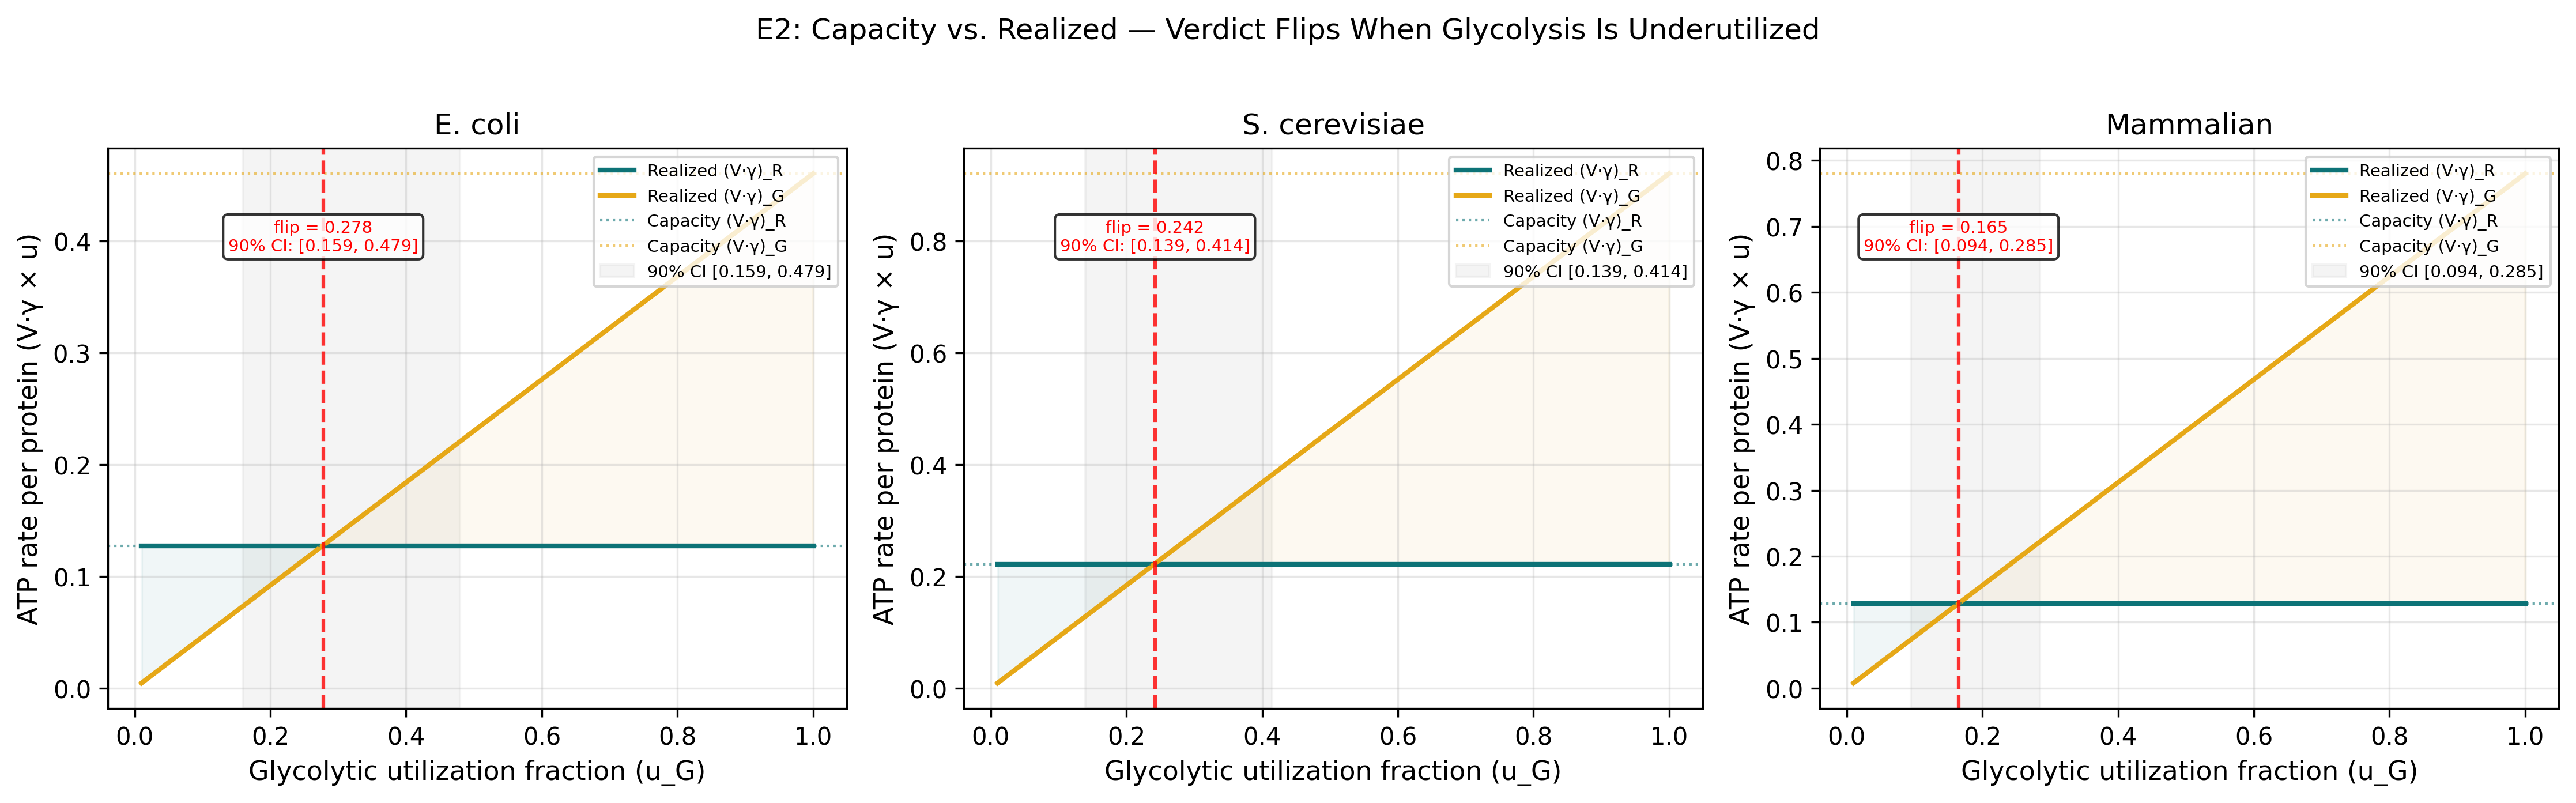
\includegraphics[width=\columnwidth]{F2_verdict_flip.png}
    \caption{E2: Efisiensi terealisasi vs.\ $u_G$. Garis merah putus-putus = titik-balik; area abu-abu = 90\% CI dari bootstrap. Hijau = respirasi menang, kuning = glikolisis menang.}
    \label{fig:e2}
\end{figure}

\subsection{E2d: Dekomposisi Atribusi Enzim}

Gambar~\ref{fig:decomp} menunjukkan bahwa reatribusi $\pm 30\%$ massa
enzim antar jalur (``enzim mana yang dihitung'') memang menggeser $\rho$
dan titik-balik, namun flip selalu mengikuti $\rho$ secara tepat.
Analisis Sobol mengkonfirmasi bahwa $u_G$ mendominasi ($S_T \approx 0{,}76$--$0{,}78$)
sementara $V_G$ dan $V_R$ masing-masing hanya berkontribusi $S_T \approx 0{,}12$.

\begin{figure}[t]
    \centering
    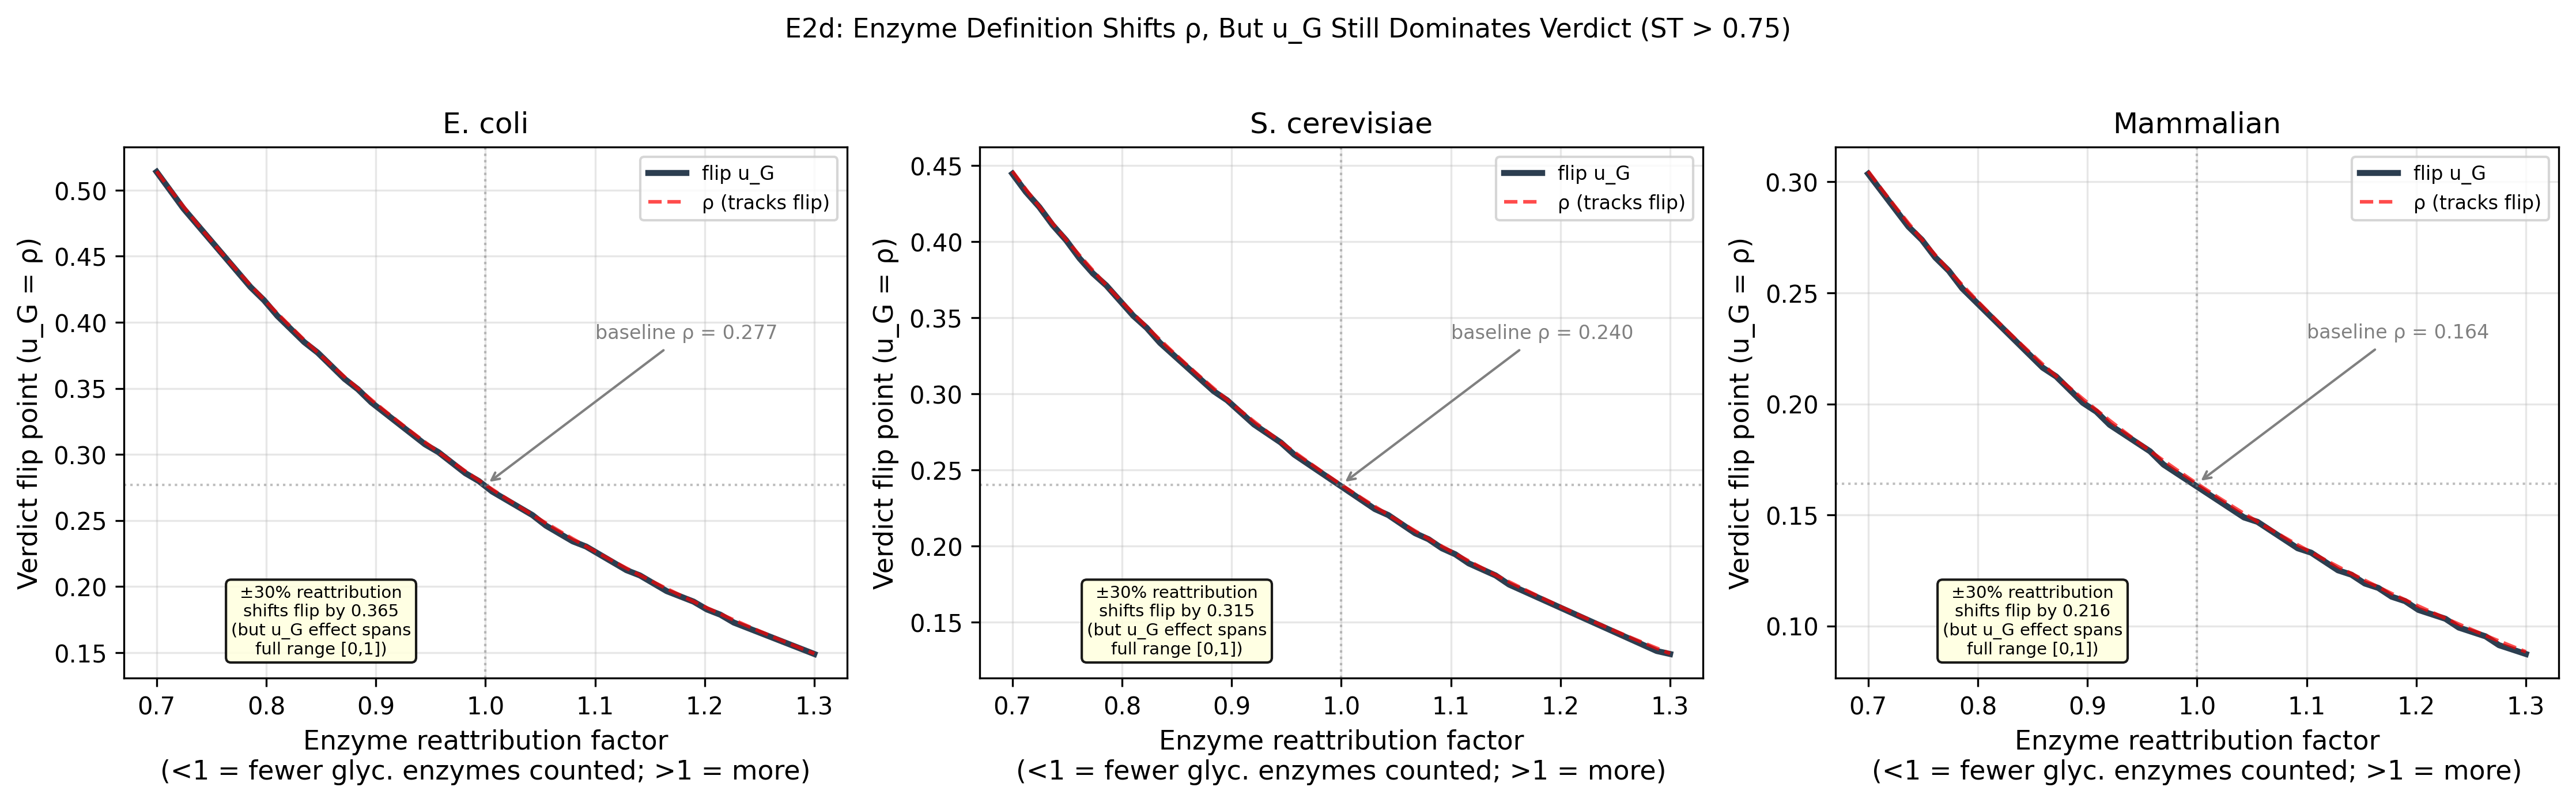
\includegraphics[width=\columnwidth]{F6_decomposition.png}
    \caption{E2d: Dekomposisi atribusi. Garis biru = flip $u_G$ terhadap faktor reatribusi enzim; garis merah putus = $\rho$ (selalu mengikuti flip). Efek reatribusi nyata namun sekunder.}
    \label{fig:decomp}
\end{figure}

\subsection{E3: Pengukuran Penuntas (Sobol/Morris)}

Gambar~\ref{fig:sobol} menampilkan indeks Sobol total-order ($S_T$)
untuk keenam parameter pada keluaran margin $m$. Untuk ketiga organisme,
$u_G$ mendominasi secara konsisten:

\begin{table}[h]
\centering
\caption{Indeks Sobol total-order ($S_T$) tiga parameter teratas (keluaran: margin $m$).}
\label{tab:sobol}
\begin{tabular}{llcc}
\toprule
\textbf{Organisme} & \textbf{Parameter} & $\boldsymbol{S_T}$ & $\boldsymbol{\pm}$ \\
\midrule
\textit{E.\ coli}    & $u_G$        & 0{,}756 & 0{,}059 \\
                      & $\gamma_G$   & 0{,}122 & 0{,}014 \\
                      & $V_G$        & 0{,}122 & 0{,}014 \\
\midrule
\textit{S.\ cerevisiae} & $u_G$     & 0{,}765 & 0{,}059 \\
                      & $\gamma_G$   & 0{,}124 & 0{,}014 \\
                      & $V_G$        & 0{,}124 & 0{,}014 \\
\midrule
Mamalia               & $u_G$        & 0{,}781 & 0{,}059 \\
                      & $\gamma_G$   & 0{,}126 & 0{,}014 \\
                      & $V_G$        & 0{,}126 & 0{,}015 \\
\bottomrule
\end{tabular}
\end{table}

Morris $\mu^*$ mengkonfirmasi peringkat yang sama (Gambar~\ref{fig:morris}).
\textbf{Temuan E3:} Pengukuran yang paling mengurangi ketidakpastian
verdict adalah $u_G$ --- fraksi pemanfaatan kapasitas glikolitik.

Namun, karena margin $m$ linier di $u_G$, dominasi ini berpotensi
tautologis. E3b menguji robustness temuan ini.

\begin{figure}[t]
    \centering
    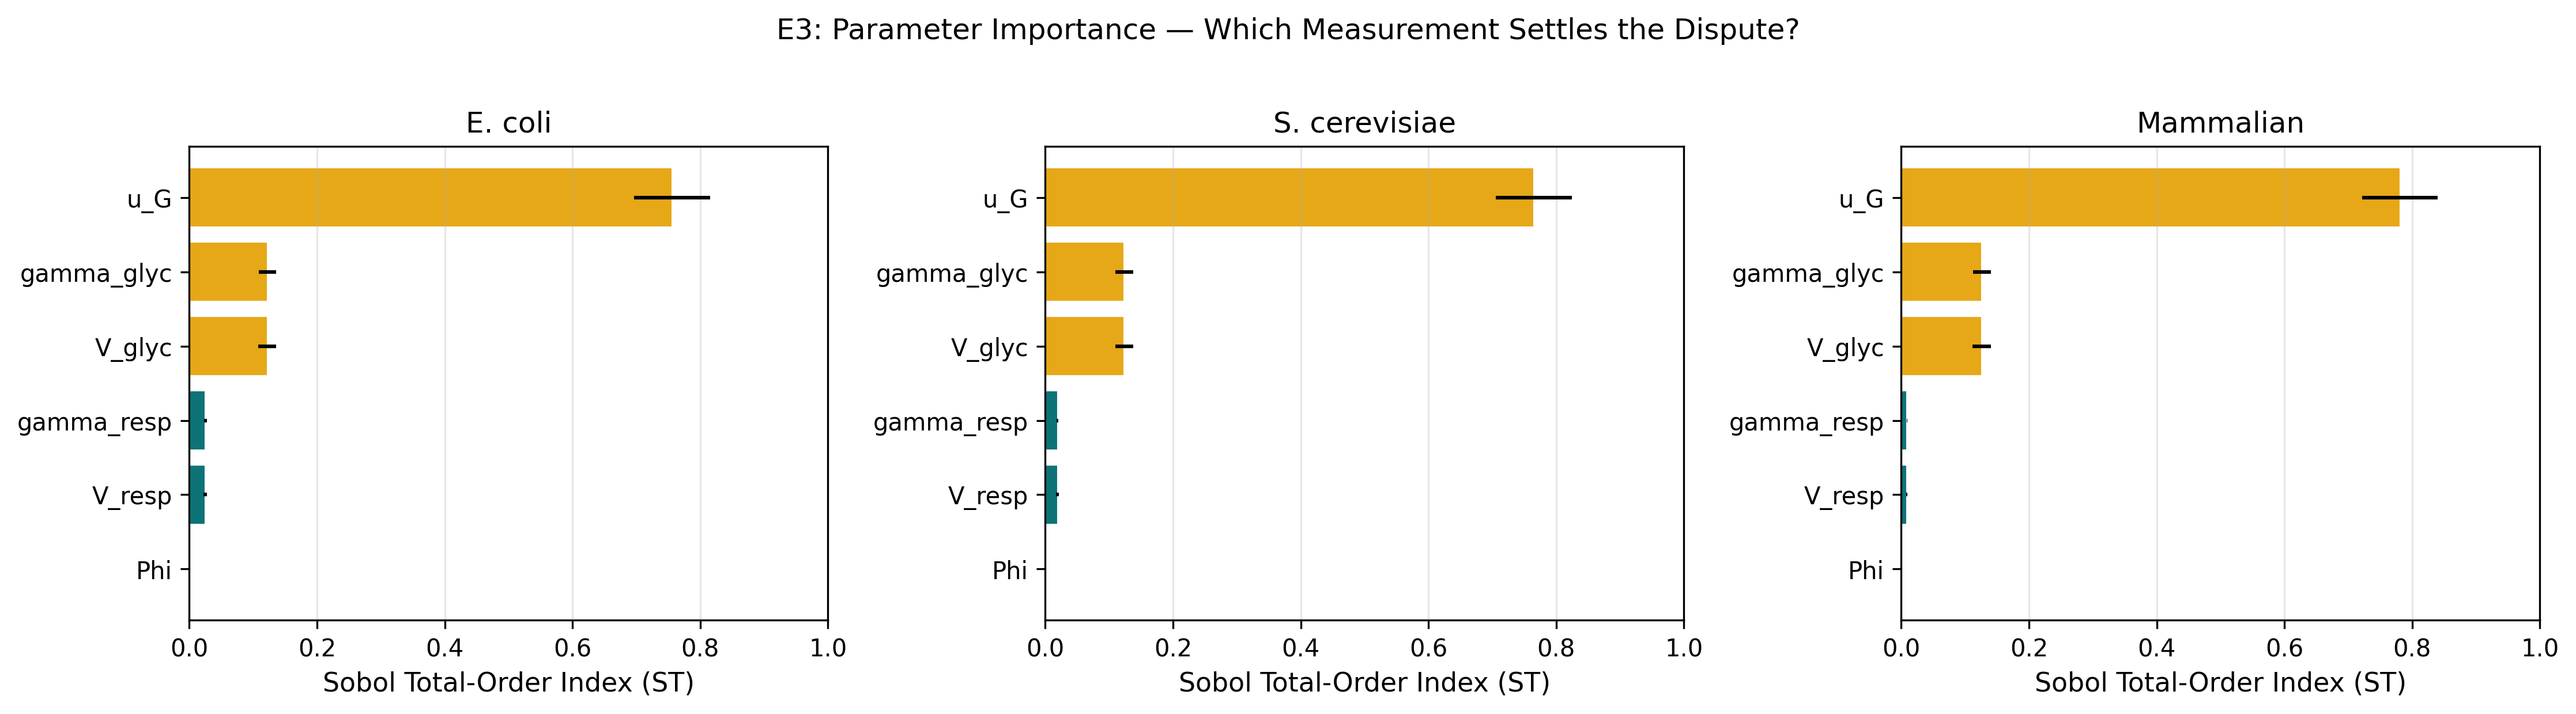
\includegraphics[width=\columnwidth]{F3_sobol_tornado.png}
    \caption{E3: Indeks Sobol total-order ($S_T$) per parameter pada keluaran margin (linier). $u_G$ mendominasi di ketiga organisme ($S_T > 0{,}75$).}
    \label{fig:sobol}
\end{figure}

\begin{figure}[t]
    \centering
    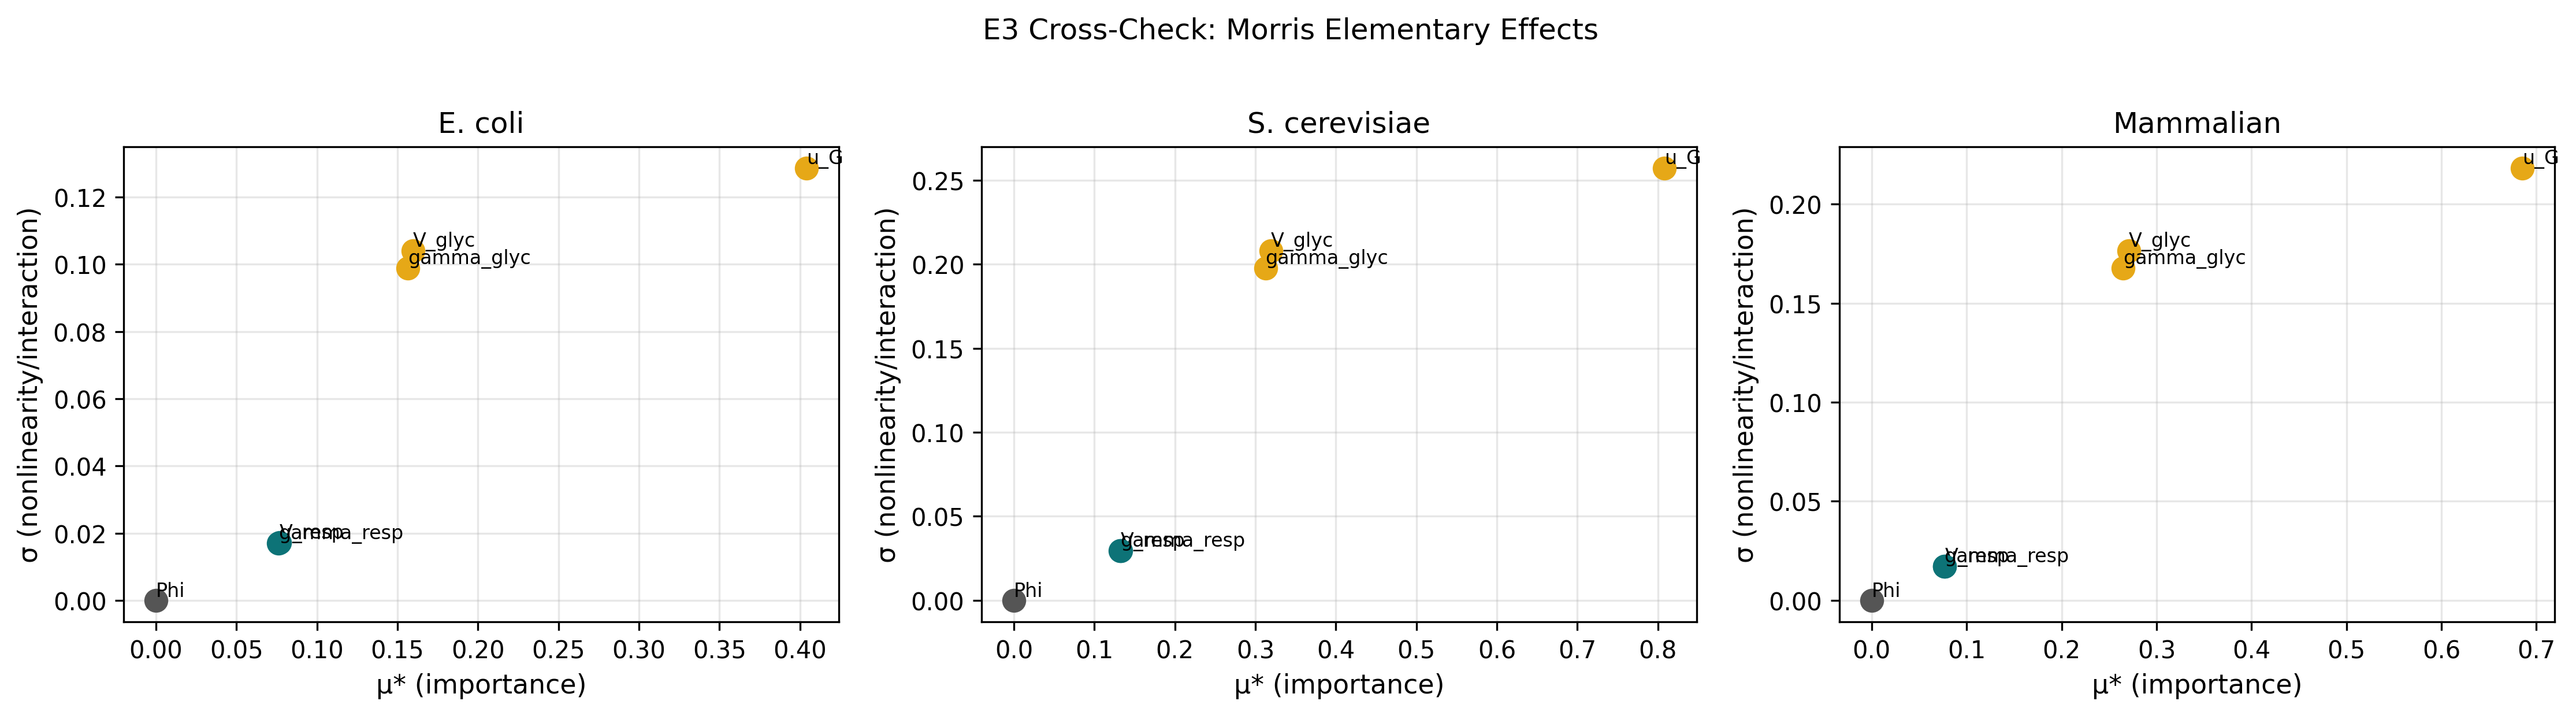
\includegraphics[width=\columnwidth]{F3b_morris_scatter.png}
    \caption{Pemeriksaan silang Morris: $\mu^*$ vs.\ $\sigma$. $u_G$ mendominasi, konsisten dengan Sobol.}
    \label{fig:morris}
\end{figure}

\subsection{E3b: Validasi Nonlinier --- Sobol pada Keluaran LP}

Gambar~\ref{fig:sobol_lp} membandingkan indeks Sobol dari keluaran
margin (linier) versus keluaran LP $f^*_G$ (nonlinier).
Pada keluaran nonlinier, kepentingan terdistribusi lebih merata:

\begin{table}[h]
\centering
\caption{Perbandingan $S_T$ teratas: margin (linier) vs.\ LP $f^*_G$ (nonlinier).}
\label{tab:sobol_lp}
\begin{tabular}{llcc}
\toprule
\textbf{Organisme} & \textbf{Parameter} & $\boldsymbol{S_T}$ \textbf{margin} & $\boldsymbol{S_T}$ \textbf{LP} \\
\midrule
\textit{E.\ coli}    & $u_G$        & 0{,}756 & 0{,}633 \\
                      & $\gamma_R$   & 0{,}017 & 0{,}301 \\
\midrule
\textit{S.\ cerevisiae} & $u_G$     & 0{,}765 & 0{,}606 \\
                      & $\gamma_R$   & 0{,}017 & 0{,}343 \\
\midrule
Mamalia               & $\gamma_R$   & 0{,}017 & \textbf{0{,}429} \\
                      & $u_G$        & 0{,}781 & 0{,}395 \\
\bottomrule
\end{tabular}
\end{table}

\textbf{Temuan E3b:} Pada keluaran nonlinier, $u_G$ tetap mendominasi
untuk \textit{E.\ coli} dan ragi, namun untuk sel mamalia
\textbf{$\gamma_R$ mengambil alih peringkat pertama} ($S_T = 0{,}43$
vs.\ $0{,}40$). Ini menunjukkan bahwa (i)~dominasi $u_G$ pada E3 bukan
sepenuhnya tautologis --- ia memang penting secara nonlinier, namun
(ii)~yield ATP respirasi ($\gamma_R$) juga merupakan pengukuran
penuntas yang kritis, terutama untuk sel mamalia. Temuan ini tidak
terlihat dari analisis margin linier.

\begin{figure}[t]
    \centering
    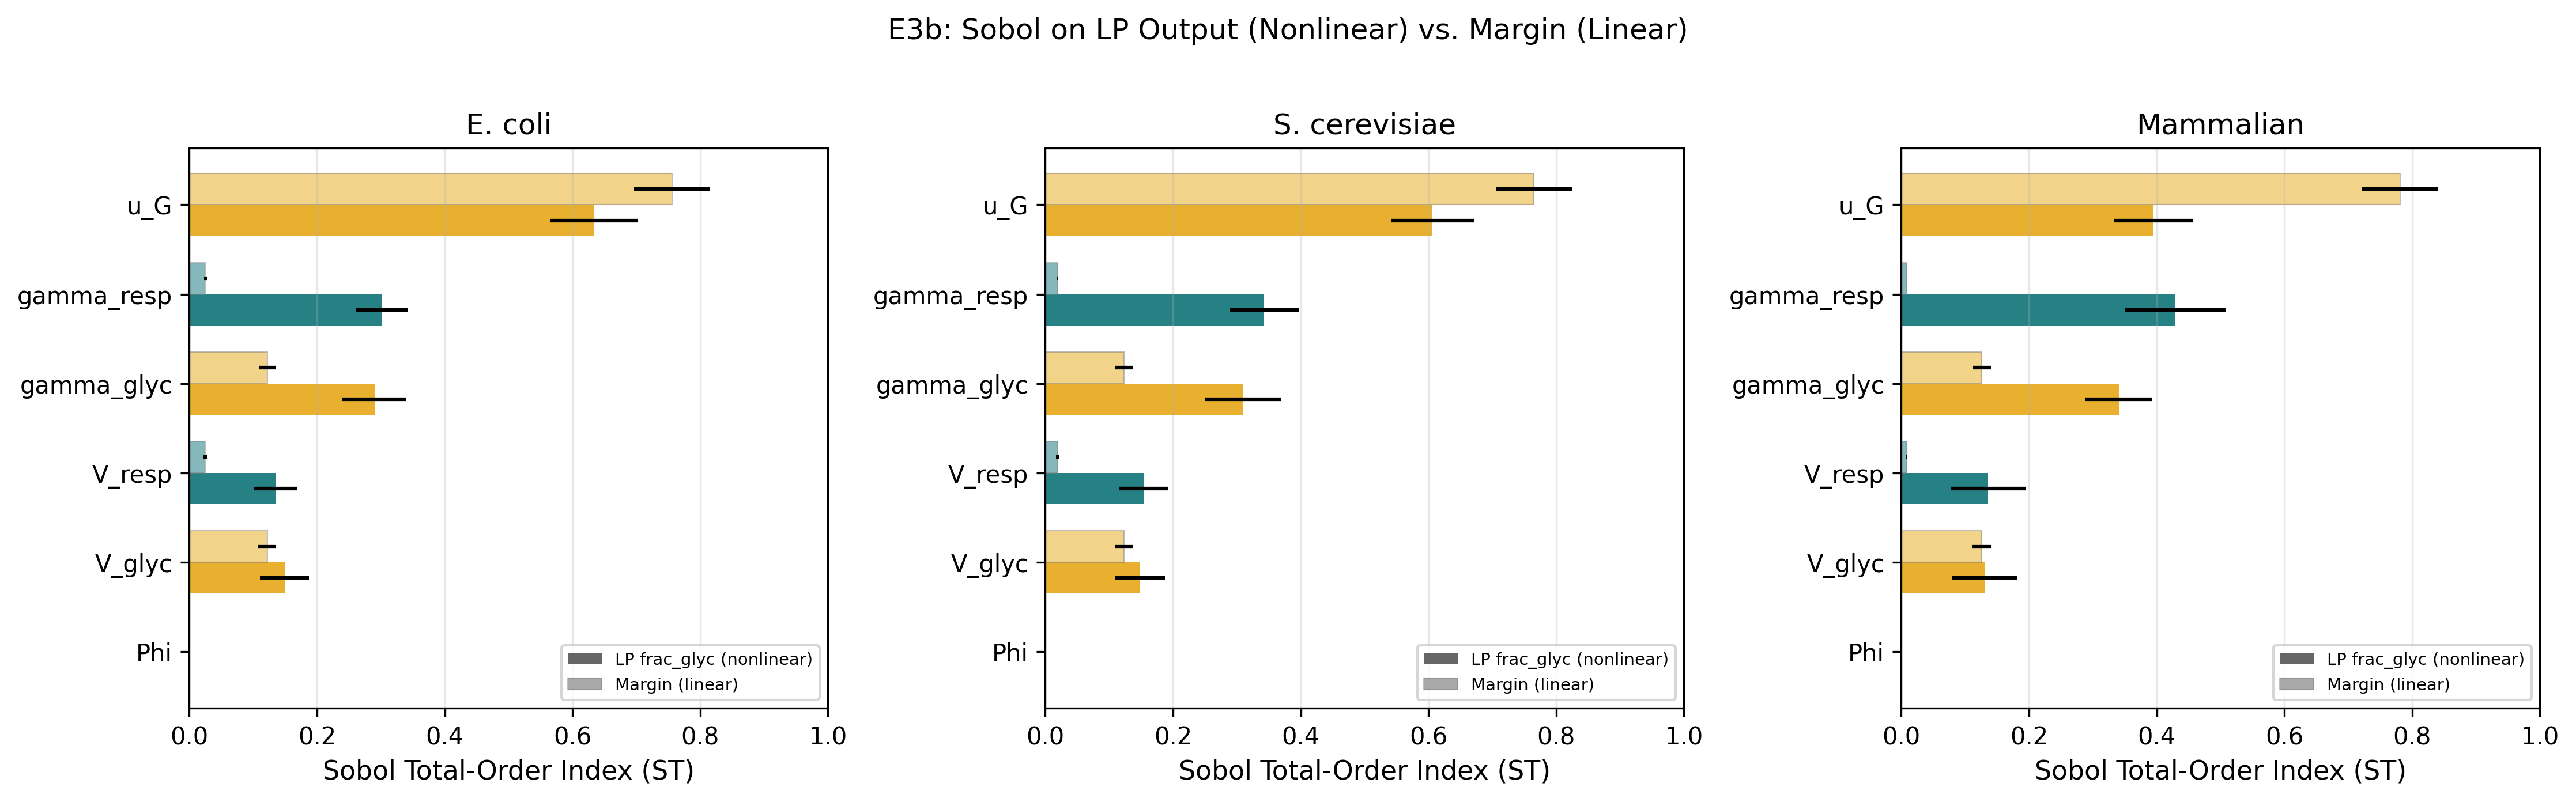
\includegraphics[width=\columnwidth]{F3c_sobol_lp.png}
    \caption{E3b: Perbandingan $S_T$ antara keluaran margin (linier, bar terang) dan keluaran LP $f^*_G$ (nonlinier, bar gelap). Pada keluaran nonlinier, $\gamma_R$ muncul sebagai parameter penting kedua.}
    \label{fig:sobol_lp}
\end{figure}

\subsection{E4: Diagram Fase Metabolik}

Gambar~\ref{fig:phase} menampilkan peta rezim 2D pada sumbu
$(g_\text{avail}, u_G)$ untuk ketiga organisme. Tiga rezim terlihat
jelas: (i)~respirasi dominan (teal, kiri bawah --- glukosa rendah),
(ii)~glikolisis dominan (kuning, kanan atas --- glukosa tinggi dan
$u_G$ tinggi), dan (iii)~zona transisi sempit. Kontur $f^*_G = 0{,}5$
(garis hitam solid) menandai batas keputusan utama.

\textbf{Temuan E4:} Batas rezim bergeser ke kanan (glukosa lebih tinggi)
seiring $u_G$ menurun --- artinya sel dengan enzim glikolitik idle
memerlukan glukosa lebih banyak sebelum beralih ke fermentasi. Ini
konsisten dengan mekanisme \textit{proteome hedging} Shen: sel
mempertahankan enzim glikolitik idle sebagai cadangan, sehingga
ambang fermentasi naik.

\begin{figure}[t]
    \centering
    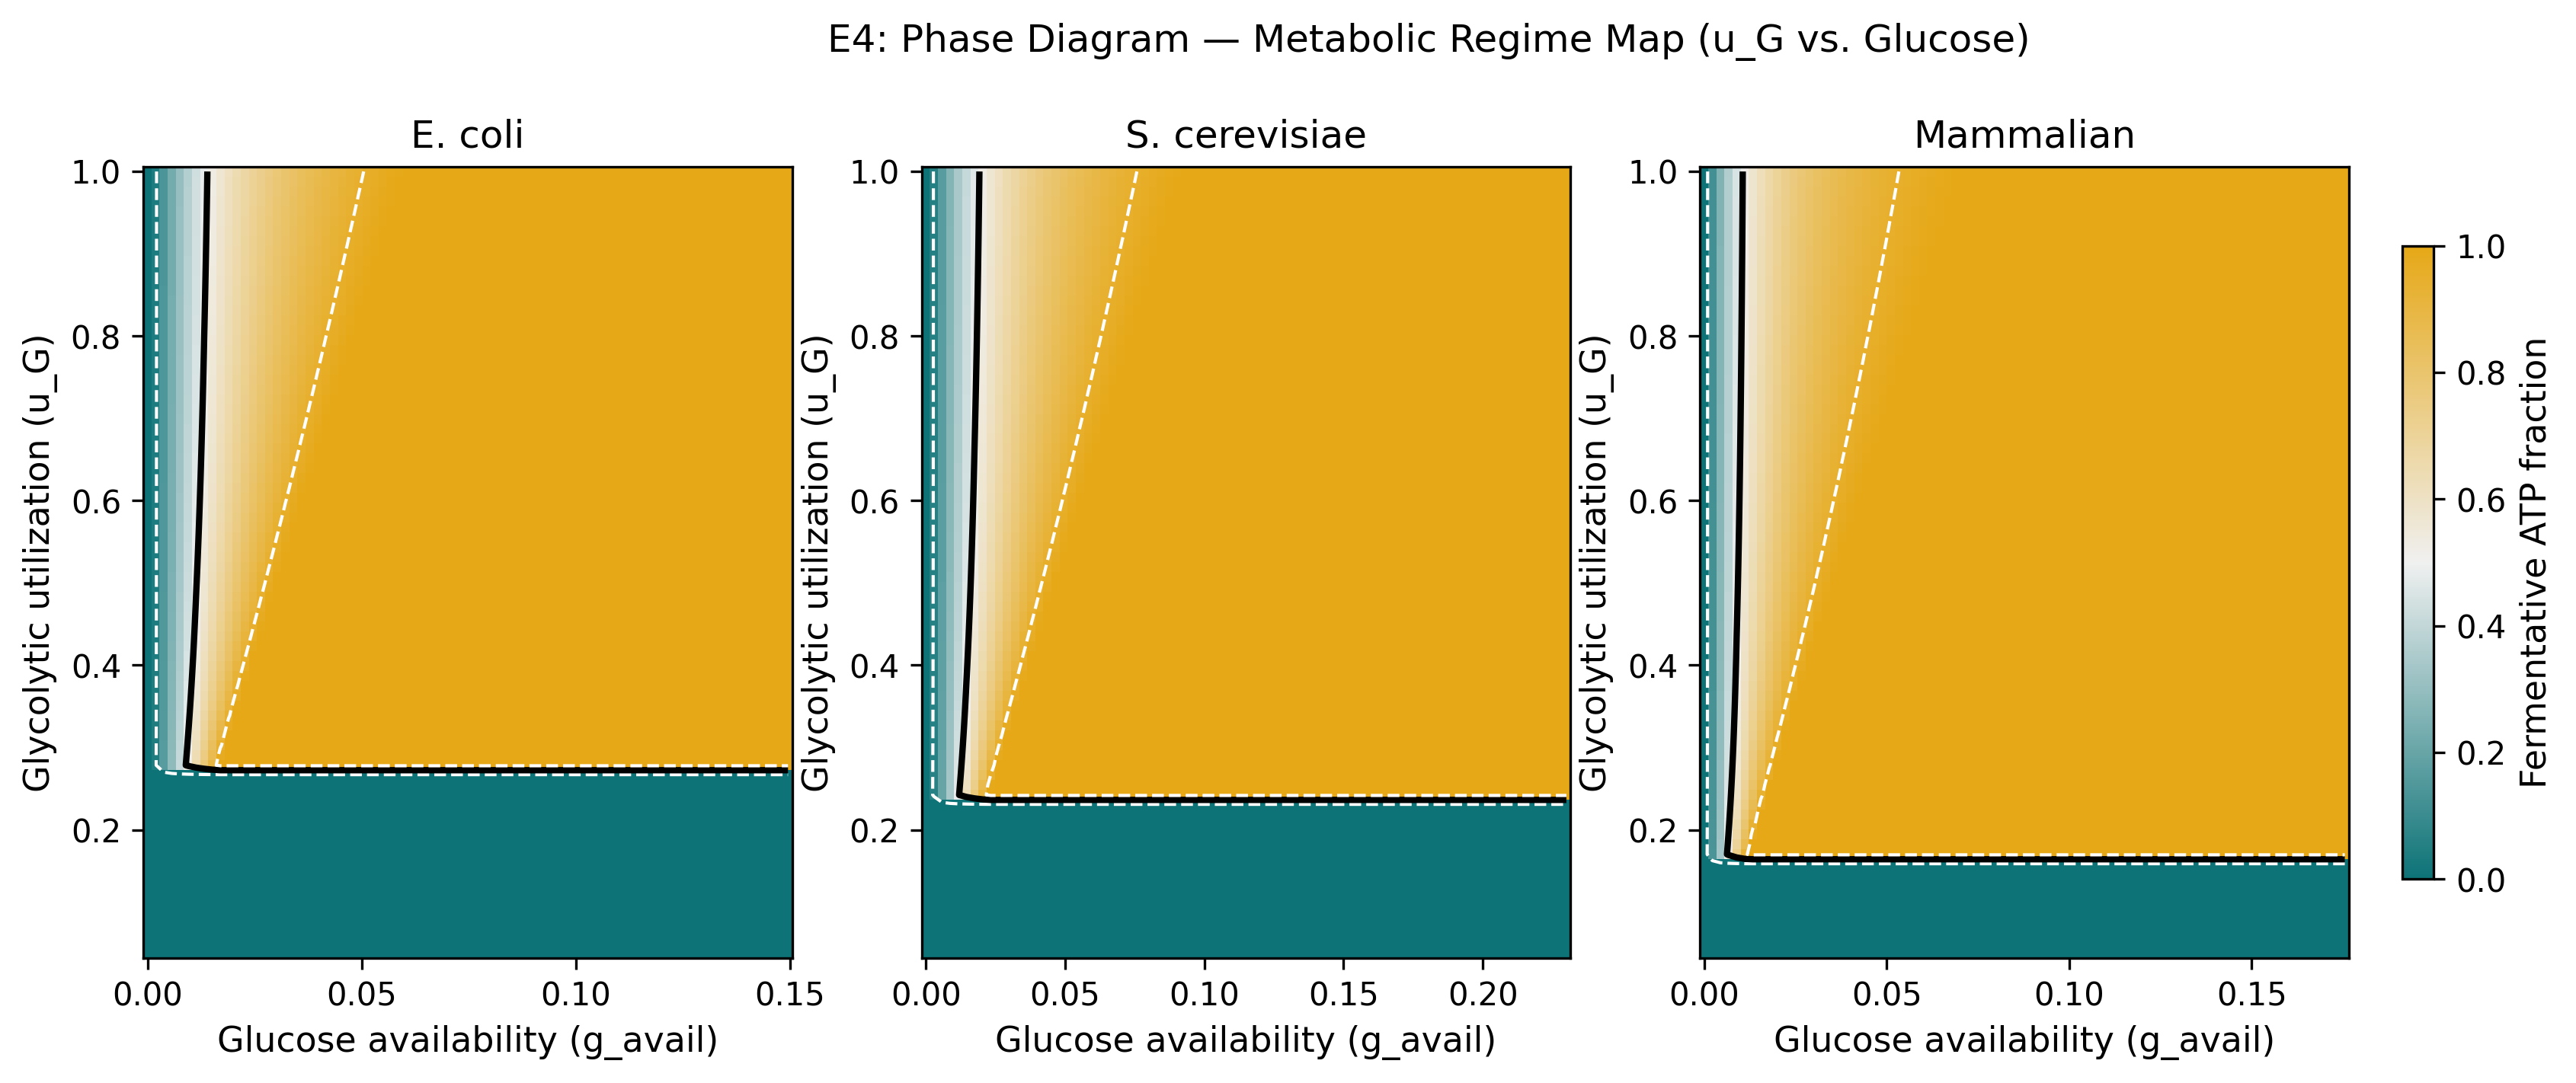
\includegraphics[width=\columnwidth]{F7_phase_diagram.png}
    \caption{E4: Diagram fase metabolik. Heatmap menunjukkan fraksi fermentatif pada grid $(g_\text{avail}, u_G)$. Kontur hitam = batas $f^*_G = 0{,}5$; putus-putus = $0{,}05$ dan $0{,}95$.}
    \label{fig:phase}
\end{figure}

\section{Diskusi}

\subsection{Interpretasi Biologis}

Temuan audit menunjukkan bahwa Shen dan Kukurugya tidak saling
bertentangan --- mereka mengukur besaran yang berbeda. Kukurugya mengukur
\textit{kapasitas maksimal} enzim ($V \cdot \gamma$), sementara Shen
mengukur \textit{efisiensi terealisasi} ($u \cdot V \cdot \gamma$) dengan
$u < 1$ karena ekspresi berlebih konstitutif protein glikolitik.

Fenomena ekspresi berlebih ini bukan artefak pengukuran: Shen melaporkan
bahwa sel mempertahankan protein glikolitik dalam jumlah besar sebagai
cadangan (``\textit{proteome hedging}'') untuk ketahanan terhadap hipoksia.
Implikasinya: pada kondisi fisiologis normal, $u_G$ rendah (banyak enzim
glikolitik idle), sehingga respirasi \textit{terlihat} lebih efisien secara
terealisasi --- persis temuan Shen. Namun, bila diukur pada kapasitas penuh
($u_G = 1$), glikolisis memang lebih cepat per protein --- persis temuan
Kukurugya.

E3b memperkuat temuan ini secara nonlinier: pada keluaran LP (bukan
rumus linier), $u_G$ tetap dominan untuk \textit{E.\ coli} dan ragi,
namun untuk mamalia $\gamma_R$ menjadi parameter terpenting --- menunjukkan
bahwa yield respirasi juga merupakan pengukuran kritis yang selama ini
terselubung oleh analisis linier. Diagram fase E4 menunjukkan bahwa
batas rezim bergeser secara kontinu dengan $u_G$, mengkonfirmasi
bahwa efek \textit{proteome hedging} beroperasi di seluruh rentang
ketersediaan glukosa.

\subsection{Posisi terhadap Wang 2025}

Gambar~\ref{fig:wang} membandingkan kerangka kami dengan Wang secara visual.
Wang memodelkan penyilangan efisiensi sebagai fungsi kualitas nutrisi $q$
--- pada $q$ tinggi respirasi menang, pada $q$ rendah fermentasi menang.
Dalam kerangka kami, variabel yang setara adalah $u_G$: kualitas nutrisi
tinggi $\leftrightarrow$ sel tumbuh lambat $\leftrightarrow$ $u_G$ rendah
(kapasitas glikolitik idle).

Kedua kerangka memprediksi titik penyilangan yang sama tetapi dari sudut
mekanistik yang berbeda. Wang memperkenalkan heterogenitas sel sebagai
mekanisme pendamaian; kami mengidentifikasi $u_G$ sebagai variabel tunggal
yang menggerakkan penyilangan tanpa perlu model heterogenitas. Keduanya
\textbf{komplementer}: Wang menjelaskan \textit{mengapa} $u_G$ bervariasi
antar-sel (heterogenitas), kami menunjukkan bahwa $u_G$ saja cukup untuk
menjelaskan perbedaan verdict.

\begin{figure}[t]
    \centering
    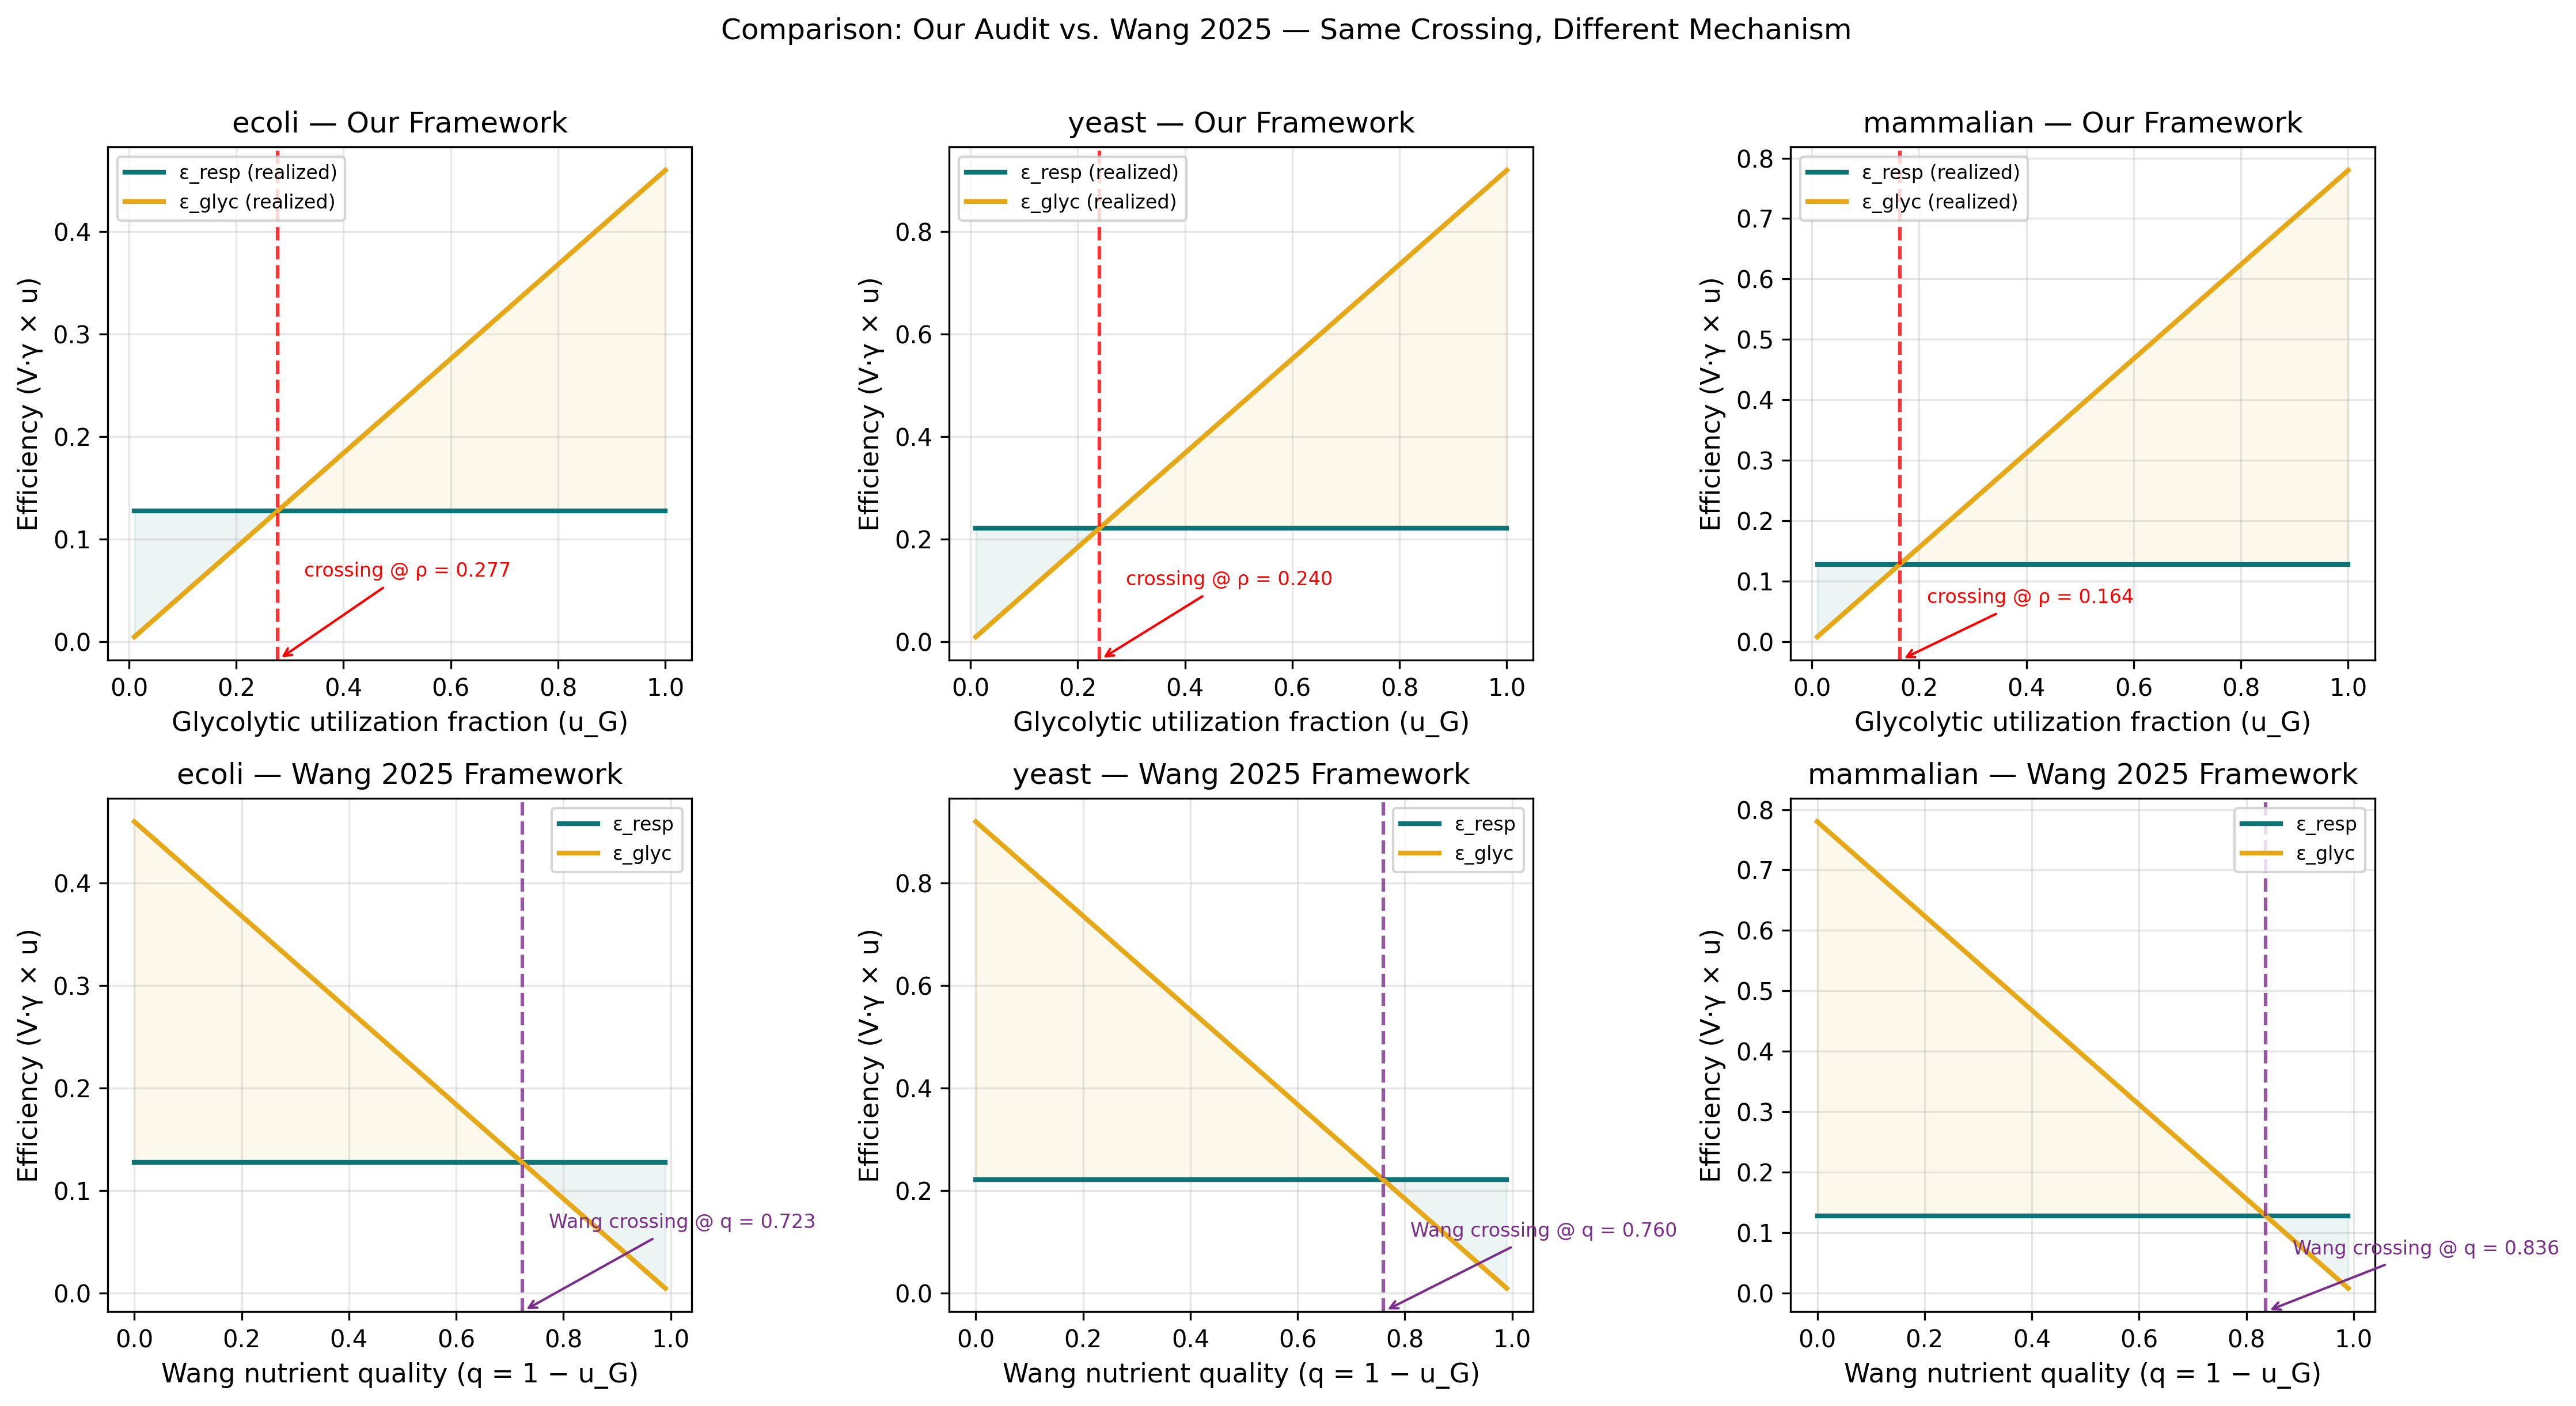
\includegraphics[width=\columnwidth]{F5_wang_comparison.png}
    \caption{Perbandingan kerangka: baris atas = sumbu $u_G$ kami, baris bawah = sumbu kualitas nutrisi $q$ Wang. Titik penyilangan sama, mekanisme berbeda.}
    \label{fig:wang}
\end{figure}

\subsection{Validasi Mekanistik (M6, Peregangan)}

Sebagai validasi tambahan, kami menambahkan kendala massa-enzim pada model
\textit{e\_coli\_core} via COBRApy (Gambar~\ref{fig:eccore}). Ketika
anggaran proteom $\Phi$ diperketat, model FBA menunjukkan onset sekresi
asetat (metabolisme limpahan) --- secara kualitatif konsisten dengan
prediksi model mainan bahwa keterbatasan proteom mendorong transisi
respirasi$\to$fermentasi.

\begin{figure}[t]
    \centering
    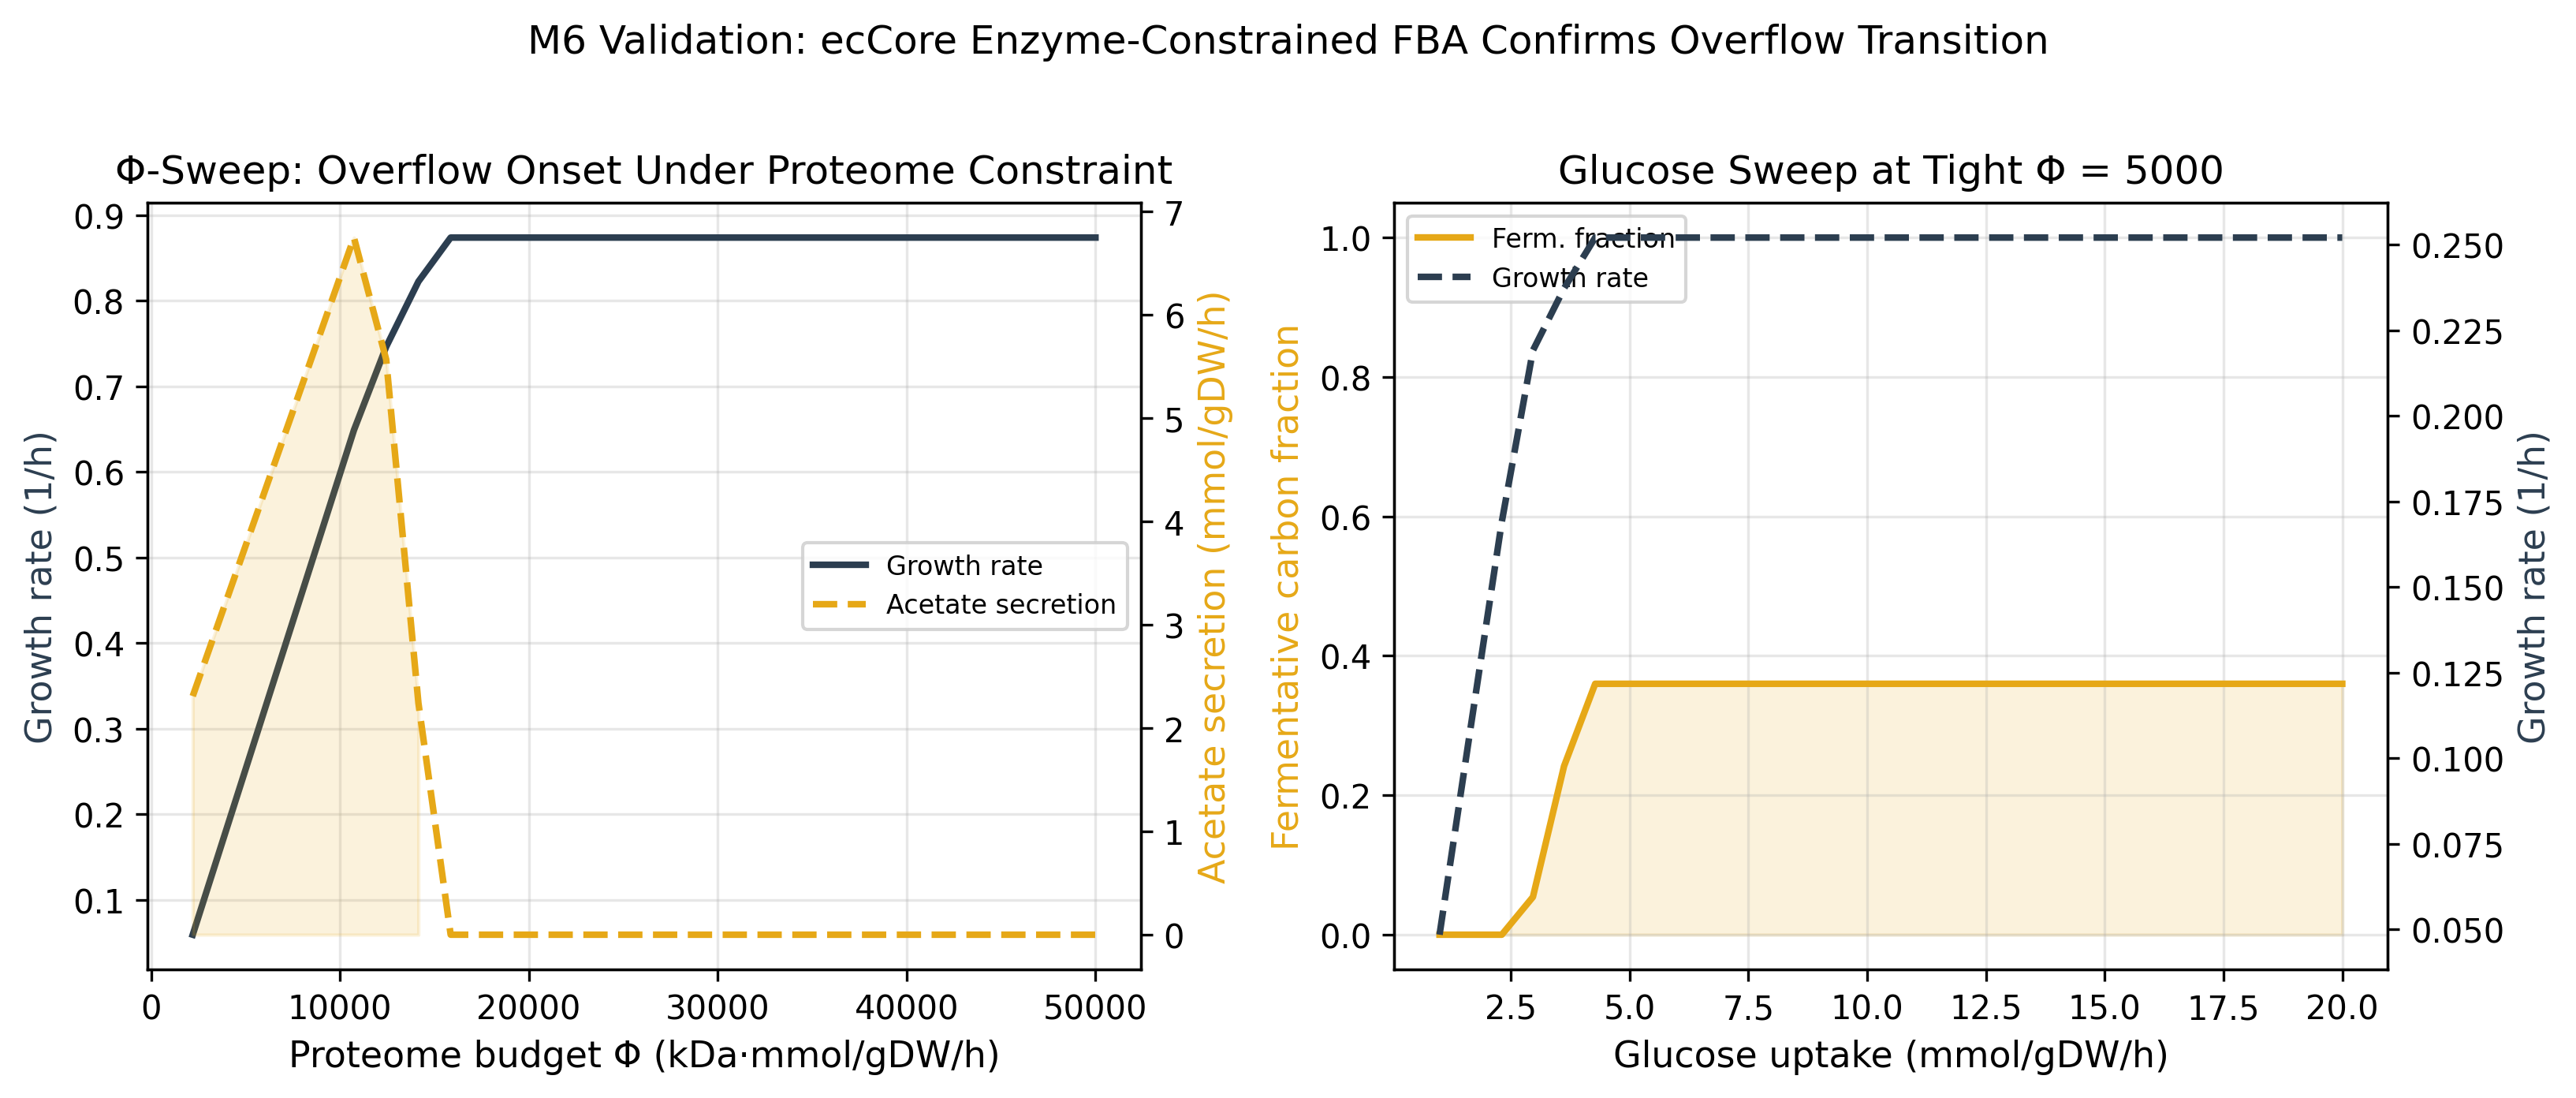
\includegraphics[width=\columnwidth]{F4_eccore.png}
    \caption{M6: FBA berbatas-enzim pada \textit{e\_coli\_core}. Kiri: penyapuan $\Phi$ menunjukkan onset limpahan asetat. Kanan: penyapuan glukosa pada $\Phi$ ketat menunjukkan peningkatan fraksi fermentatif.}
    \label{fig:eccore}
\end{figure}

\subsection{Keterbatasan}

Beberapa keterbatasan perlu diakui:
\begin{enumerate}
    \item \textbf{Model \textit{coarse-grained}.} Kedua model adalah
          penyederhanaan dua-sektor; model skala-genom (GECKO, ETFL) akan
          memberikan resolusi lebih tinggi.
    \item \textbf{Parameter provisional.} Nilai parameter ditandai
          PROVISIONAL dan berasal dari ringkasan tabel, bukan pengukuran
          langsung kami. Verifikasi dari SI asli diperlukan.
    \item \textbf{Tiga organisme saja.} Audit terbatas pada
          \textit{E.\ coli}, ragi, dan sel mamalia; generalisasi ke
          organisme lain belum teruji.
    \item \textbf{In-silico.} Seluruh temuan bersifat komputasional;
          validasi eksperimental (pengukuran $u_G$ in-vivo) diperlukan.
\end{enumerate}

\section{Kesimpulan}

Audit komputasi ini menunjukkan bahwa perselisihan Shen--Kukurugya 2024
bersumber terutama pada \textbf{besaran yang diukur} (kapasitas $V\!\cdot\!\gamma$
versus efisiensi terealisasi $u\!\cdot\!V\!\cdot\!\gamma$), bukan pada
struktur model. Verdict membalik pada $u_G \approx \rho$ untuk ketiga
organisme --- interval kepercayaan 90\% seluruhnya di bawah 1{,}0 ---
mengkonfirmasi bahwa fraksi idle glikolitik (konsisten dengan ``\textit{proteome
hedging}'' Shen) cukup untuk menjelaskan perbedaan. Analisis sensitivitas
global Sobol mengidentifikasi $u_G$ sebagai pengukuran penuntas
($S_T \approx 0{,}76$--$0{,}78$), sementara definisi enzim berkontribusi
sekunder ($S_T \approx 0{,}12$). Mekanisme penyilangan yang kami temukan
komplementer terhadap pendamaian Wang 2025.

Untuk kerja masa depan, kami merekomendasikan: (i)~pengukuran $u_G$
in-vivo per organisme menggunakan proteomik kuantitatif berpasangan
dengan fluksomik, sebagai eksperimen penuntas; (ii)~perluasan ke model
skala-genom (GECKO/ETFL) untuk resolusi enzim-per-enzim; dan
(iii)~integrasi dengan kerangka heterogenitas Wang untuk menguji apakah
variabilitas $u_G$ antar-sel menjelaskan dispersi fenotipe metabolik
yang diamati.

Kode sumber tersedia di: \url{https://github.com/[REPO]}.


% ====================================================================
\bibliographystyle{IEEEtran}
\bibliography{references}

\end{document}
